\documentclass[13pt]{article}
\usepackage{amsmath, amsthm, amssymb, graphicx, enumitem, esvect, tikz}
\usetikzlibrary{automata, positioning, arrows}
\tikzset{
  ->,
  ->/.style={thick},
  every state/.style={thick, fill=gray!10},
  initial text=$ $,
}

% Language setting
% Replace `english' with e.g. `spanish' to change the document language
\usepackage[english]{babel}

% Set page size and margins
% Replace `letterpaper' with `a4paper' for UK/EU standard size
\usepackage[letterpaper,top=2cm,bottom=2cm,left=3cm,right=3cm,marginparwidth=1.75cm]{geometry}

\title{CS 181}
\author{Warren Kim}

\begin{document}
\maketitle

\newpage
\tableofcontents

\newpage
\section*{Preface}
In this course, we want to answer two questions:
\begin{enumerate}[label=(\arabic*),leftmargin=*]
\item What is computation?
\item Are there problems that computers cannot solve?
\end{enumerate}

\section{Deterministic Finite Automata}

\subsection{Definitions}
\begin{itemize}[label=,leftmargin=*]
\item Alphabet: Any \textbf{nonempty finite} set of symbols.
  \begin{itemize}[label=]
  \item [($\beta$)] $\{0, 1\}$ is the binary alphabet.
  \item [($\gamma$)] ${+, -, \cdot, /}$ is the alphabet of arithmetic operators.
  \item [($\alpha$)] ${a, b, \ldots, z}$ is the alphabet of lowercase English letters.
  \end{itemize}

\item String: Any \textbf{finite} sequence of symbols from a given alphabet. \\
  \textit{\textbf{Note:}} The empty string ($\epsilon$) is the only string contained in \textbf{all}
  alphabets.
  \begin{itemize}[label=]
  \item $101101 \in \beta$
  \item $++-/--\cdot-+ \in \gamma$
  \item $abcad \in \alpha$
  \end{itemize}

\item Language: A set of strings over a given alphabet. More specifically, the language of a Discrete
  Finite Automata (DFA) is a set of strings that the DFA accepts.
  \begin{enumerate}[label=(\arabic*)]
  \item $\{0, 001, 010, 100, \ldots\}$ is the set containing all odd length binary strings over $\beta$
  \item $\{aim, claim, denim, \ldots\}$ is the set containing all English words that end in "$im$" over
    $\gamma$
  \item $\{\epsilon\}$ is the set containing the empty string over \textbf{all} alphabets.
  \item $\O$ is the empty set over \textbf{all} alphabets.
  \end{enumerate}
  \textit{\textbf{Note:}} (1) and (2) are infinite while (3) and (4) are finite languages. \\

\item Computational Device: Any mechanism that imports a string and either accepts or rejects it.
  \begin{figure}[ht]
    \centering
    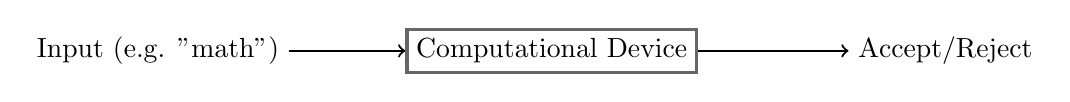
\begin{tikzpicture}[SIR/.style={rectangle, draw=black!60, very thick}]
      \node (Input) {Input (e.g. "math")};
      \node[SIR] (CompDevice) [right of=Input, xshift=4cm] {Computational Device};
      \node (Output) [right of=CompDevice, xshift=4cm] {Accept/Reject};

      \draw[->, thick] (Input.east) to node[right] {} (CompDevice.west);
      \draw[->, thick] (CompDevice.east) to node[right] {} (Output.west); 
    \end{tikzpicture}
  \end{figure}
\end{itemize}





\subsection{Formulating Automata}
Automata abides by the following rules:
\begin{itemize}
\item Choose an alphabet.
\item Draw states.
\item Choose a start\footnote{Start states are required} state.
\item Choose accept\footnote{Accept states are \textbf{not} required} states.
\item Draw transitions from \textbf{every} state to \textbf{every} symbol.
\end{itemize}

\newpage
\subsubsection{Automata Examples}
\begin{figure}[ht]
  \centering
  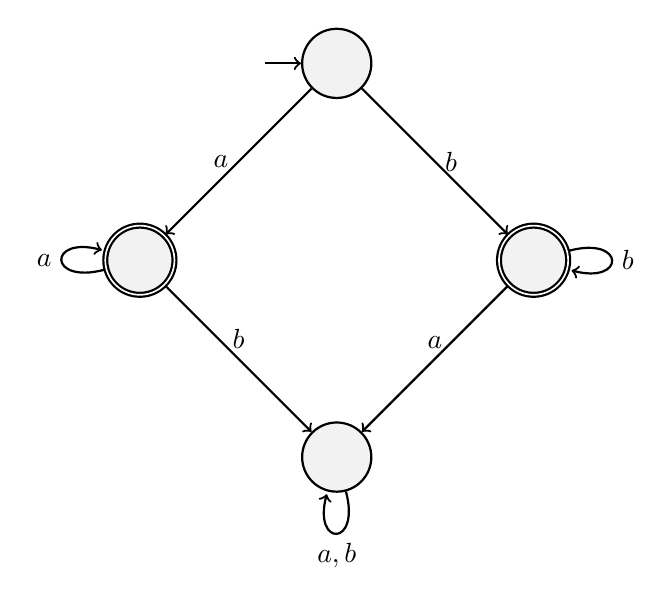
\begin{tikzpicture}
    \node[state, initial] (init) {};
    \node[state, accepting, xshift=-2.5cm, yshift=-2.5cm] (q1) {};
    \node[state, accepting, xshift=2.5cm, yshift=-2.5cm] (q2) {};
    \node[state, yshift=-5cm] (q3) {};

    \draw (init) edge[->, left] node{$a$} (q1);
    \draw (init) edge[->, right] node{$b$} (q2);

    \draw (q1) edge[loop left] node{$a$} (q1);
    \draw (q1) edge[->, above] node{$b$} (q3);

    \draw (q2) edge[loop right] node{$b$} (q2);
    \draw (q2) edge[->, above] node{$a$} (q3);

    \draw (q3) edge[loop below] node{$a, b$} (q3);
  \end{tikzpicture}
  \caption{Accepts the set of strings $W = \{w : w \text{ is nonempty and contains either all $a$'s or
    all $b$'s}\}$ over the alphabet $\{a, b\}$}
\end{figure}

\begin{figure}[ht]
  \centering
  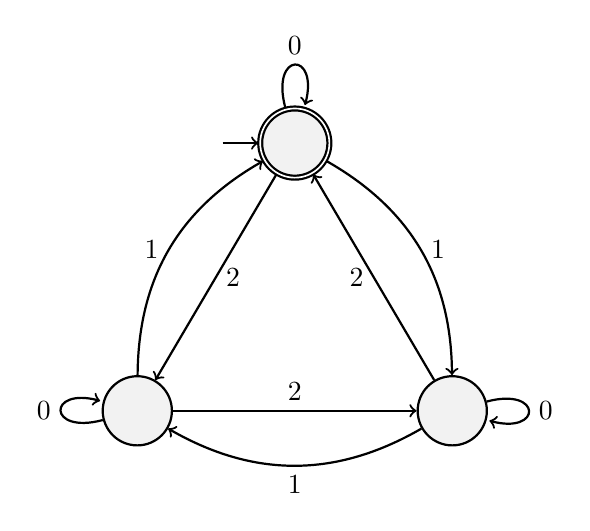
\begin{tikzpicture}
    \node[state, initial, accepting] (init) {};
    \node[state, xshift=-2cm, yshift=-3.4cm] (q1) {};
    \node[state, xshift=2cm, yshift=-3.4cm] (q2) {};   

    \draw (init) edge[loop above] node{$0$} (init);
    \draw (init) edge[->, bend left, right] node{$1$} (q2);
    \draw (init) edge[->, right] node{$2$} (q1);

    \draw (q1) edge[loop left] node{$0$} (q1);
    \draw (q1) edge[->, bend left, left] node{$1$} (init);
    \draw (q1) edge[->, above] node{$2$} (q2);

    \draw (q2) edge[loop right] node{$0$} (q2);
    \draw (q2) edge[->, bend left, below] node{$1$} (q1);
    \draw (q2) edge[->, left] node{$2$} (init);
  \end{tikzpicture}
  \caption{Accepts the set of strings $W = \{w : w \text{ is nonempty and } \sum_{i = 1}^{k = |w|}
    w_{i} \text{ is divisible by 3, } 1 \leq i \leq n\}$ over the alphabet $\{0, 1, 2\}$}
\end{figure}

\begin{figure}[ht]
  \centering
  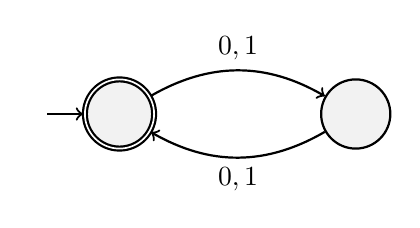
\begin{tikzpicture}
    \node[state, initial, accepting] (init) {};
    \node[state, xshift=3cm] (q1) {};

    \draw (init) edge[->, bend left, above] node{$0, 1$} (q1);

    \draw (q1) edge[->, bend left, below] node{$0, 1$} (init);
  \end{tikzpicture}
  \caption{Accepts the set of strings $W = \{w : |w| \text{ is even, } 1 \leq i \leq n\}$ over the
  alphabet $\{0, 1\}$}
\end{figure}

\begin{figure}[ht]
  \centering
  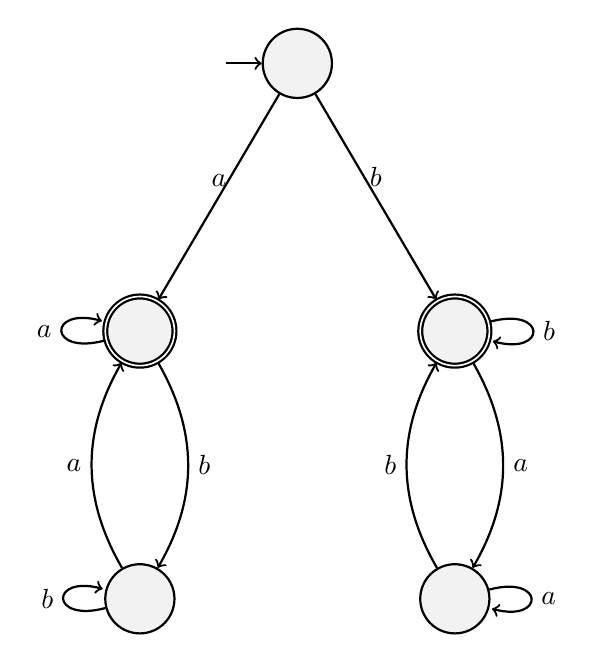
\begin{tikzpicture}
    \node[state, initial] (init) {};
    \node[state, accepting, xshift=-2cm, yshift=-3.4cm] (q1) {};
    \node[state, accepting, xshift=2cm, yshift=-3.4cm] (q2) {};
    \node[state, xshift=-2cm, yshift=-6.8cm] (q3) {};
    \node[state, xshift=2cm, yshift=-6.8cm] (q4) {};
    
    \draw (init) edge[->, above] node{$a$} (q1);
    \draw (init) edge[->, above] node{$b$} (q2);

    \draw (q1) edge[loop left] node{$a$} (q1);
    \draw (q1) edge[->, bend left, right] node{$b$} (q3);

    \draw (q2) edge[loop right] node{$b$} (q2);
    \draw (q2) edge[->, bend left, right] node{$a$} (q4);

    \draw (q3) edge[loop left] node{$b$} (q3);
    \draw (q3) edge[->, bend left, left] node{$a$} (q1);
    
    \draw (q4) edge[loop right] node{$a$} (q4);
    \draw (q4) edge[->, bend left, left] node{$b$} (q2);
  \end{tikzpicture}
  \caption{Accepts the set of strings $W = \{w : w \text{ is nonempty and begins and ends with
      the same letter, } 1 \leq i \leq n\}$ over the alphabet $\{a, b\}$}
\end{figure}
\end{document}

%%% Local Variables:
%%% mode: latex
%%% TeX-master: t
%%% End:
